\chapter{Particle-in-Cell Simulations of Enhanced Target Normal Sheath Acceleration} \label{ch:4}

This chapter details the work I did in conducting PIC simulations to better understand the Enhanced Target Normal Sheath Acceleration (eTNSA) mechanism that our group tried to demonstrate using LLNL's Titan Laser in March of 2024. As a result, I will mostly focus on the simulation aspect, but include some relevant comparisons to the experiment. 

\section{Theory}

\subsection{Spatially Aligned Pulses} \label{sec:spatialalign}

\begin{figure}
	\centering 
	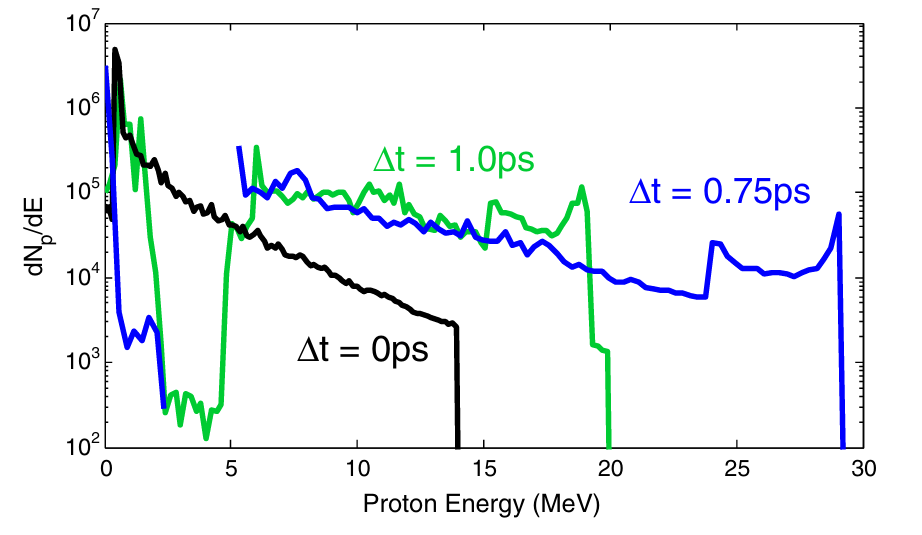
\includegraphics[width=0.75\linewidth]{planning/images/Markey_Spectrum.PNG}
	\caption{Proton energy spectrum from 1D PIC simulations depicted for three different temporal delays (including $\Delta t = 0$) from FIG. 3 in Markey et. al.\cite{Markey_2010_PRL}.}
	\label{fig:markey_spectrum}
\end{figure}

As explained in \cref{sec:tnsa_opt}, there is generally an optimal level of pre-expansion of the target to maximize the TNSA proton energies\cite{McKenna_2008_LaPB,Fuchs_2007_PRL}. While this could be attributed to a low contrast pulse, this could also be an artificially injected pre-pulse whose intensity and temporal delay are tunable. Robinson et. al.\cite{Robinson_2007_PPCF} first addresses the idea of using multiple high intensity 40 fs laser pulses with the first being one-tenth to one-quarter of the intensity of the second. They termed this novel two-stage process ``multiple pulse sheath acceleration''. This study actually found a reduction in peak proton energy through numerical simulations, but did find the existence of ``spectral peaks'' -- spikes in the energy spectrum as specific energies. A few years later, Markey et. al.\cite{Markey_2010_PRL} examined a similar setup experimentally, varying the temporal separation by 0.75-2.5 ps. Interestingly, they found an enhancement in the peak proton energy with a 0.75 ps separation and pulse energy ratio of 0.4:1. They conducted 1D PIC simulations shown in \cref{fig:markey_spectrum} that verify this as well.

In 2018, Ferri et. al.\citep{Ferri_2018_PoP} re-examines the same question, but uses the same intensity for both pulses. He finds that ultimately, little to no delay is optimal and as the delay gets larger, the enhancement reduces to the single pulse result. He finds the acceleration process can be affected by the second pulse for time delays as long as $\SI{0.6}{\pico \second}$ for $\SI{3}{\micro \meter}$ targets and $\SI{1}{\pico \second}$ for $\SI{6}{\micro \meter}$ targets. 

In a different approach Scott et. al. \cite{Scott_2012_APL} realized that much of the laser light that is reflected is wasted, so a mechanism to re-direct this light back into the target would be desired. They designed a target with a half-cavity foil as seen in \cref{fig:scott_half_cavity} that will take light reflected off the accelerating foil and re-reflect it back towards the accelerating foil. They find that this can increase the laser to proton energy efficiency by up to $\sim 55 \%$.

\begin{figure}
	\centering 
	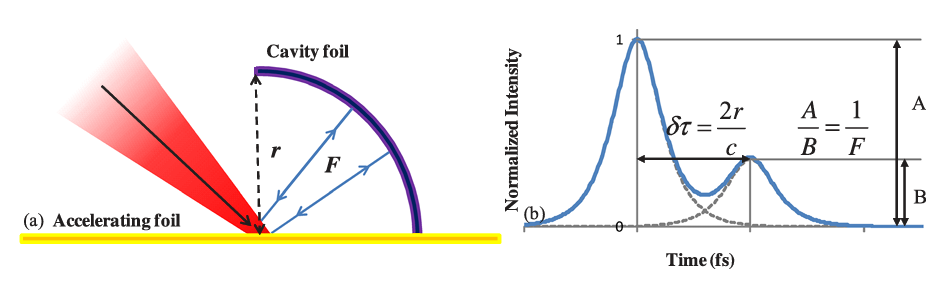
\includegraphics[width=0.75\linewidth]{planning/images/scott_half_cavity.PNG}
	\caption{Schematic of the incident laser on the half-cavity target (left) in Scott et. al.\cite{Scott_2012_APL}. The radius of the cavity foil determines the delay ($\tau = 2 r/c$) between the main pulse and the post-pulse (reflected laser light of $\sim 40 \%)$ energy of the main pulse).}
	\label{fig:scott_half_cavity}
\end{figure}

%Since we're looking at a 15 micron target, I'd imagine this time would be around 2ps, but I could solve his equations to get a better estimate. This time coincides when the fastest ions have moved a distance of the order of the transverse extent of the electric sheath field.

%Explain what contrast is: peak of the laser pulse compared to the pedestal and maybe give a diagram.

\subsection{Spatially and Temporally Aligned Pulses}

\subsubsection{Ferri}
Given the results of the previous section\cite{Markey_2010_PRL,Scott_2012_APL,Ferri_2018_PoP} that use short-delay pre or post pulses, Ferri decided to study how a spatially \emph{and} temporally aligned pulse can enhance proton acceleration. Ferri, Siminos, and Fulop showed that the double pulse setup can result in an almost doubling of the proton energy and five-fold enhancement in the number of protons\cite{Ferri_2019_Nat_Comm} through PIC simulations. This phenomena, referred to as eTNSA, is depicted in \cref{fig:ferri_dub_pulse} which shows the constructive interference of the fields at the front of the target in the center panel (e) and enhanced TNSA fields at the target rear (f).

\begin{figure}
	\centering 
	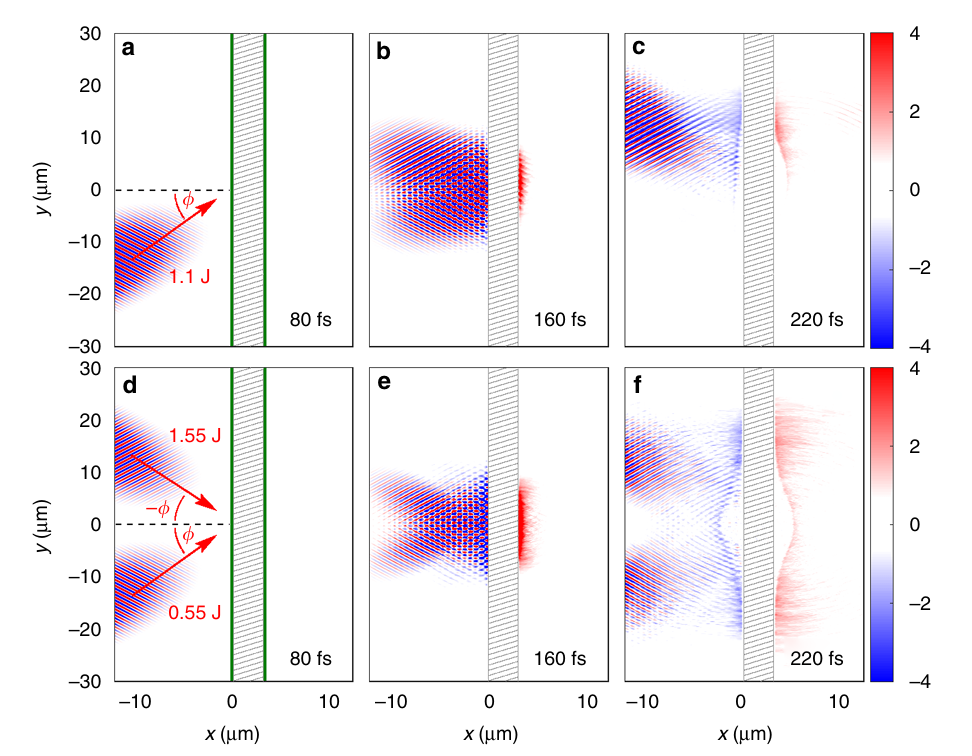
\includegraphics[width=\linewidth]{planning/images/ferri_dub_pulse.PNG}
	\caption{Geometry of the two pulse scheme as shown in FIG. 1 of Ferri et. al. (2019)\cite{Ferri_2019_Nat_Comm}. The single pulse has a total energy of 1.1J at an incidence angle of $\phi=45^\circ$ and is shown through several time snapshots (a-c). In (d-f), the double pulse is shown through those same time snapshots with energies of 0.55 J in each pulse (the 1.55 J is a typo from the original figure). Other parameters includde $\tau_\text{fwhm} = \SI{38}{\femto \second}$, thickness = $\SI{3}{\micro \meter}$, material = aluminum, $w_\text{0,fwhm} = \SI{5}{\micro \meter}$, $I_0 = \SI{7e19}{\watt \per \centi \meter \squared}$.}
	\label{fig:ferri_dub_pulse}
\end{figure}
The constructive interference of the electric fields can be understood by considering the electric field of two p-polarized pulses coming in at angles of incidence $\phi$ and $-\phi$

\begin{align}
	E_{x,1} &= -E_0 \sin(\phi) \sin(k y \sin(\phi) - \omega t + k x \cos(\phi)) \\
	E_{x,2} &= -E_0 \sin(\phi) \sin(k y \sin(\phi) - \omega t - k x \cos(\phi))
\end{align}
Adding these two fields together results in 

\begin{equation}
	E_\text{double} = -2 E_0 \sin(\phi) \sin(k y \sin(\phi) - \omega t) \cos(k x \cos(\phi))
\end{equation}
which has an amplitude of $\lvert E_\text{double} \rvert = 2 E_0 \sin(\phi)$. In contrast, a single pulse with twice the energy (intensity) would only have a $\sqrt{2}$ larger electric field ($\lvert E_\text{single} \rvert = \sqrt{2} E_0 \sin(\phi)$) which explains the enhanced electric fields seen in the bottom row of \cref{fig:ferri_dub_pulse}. In an ideal situation where 100 \% of the laser pulse is reflected, the angles of the two pulses do not need to be equal and opposite -- we will get a standing wave pattern from the constructive interference of the incident wave with its reflection and the same $\sqrt{2}$ field enhancement.  

Unlike the methods described in \cref{sec:spatialalign} (which see enhanced proton acceleration from a pre-expanded target), eTNSA relies on the presence of an undisturbed target from the vacuum heating mechanism\cite{Brunel_1987_PRL} explained in \cref{sec:absorption}. Vacuum heating relies on the dominance of the electron's quiver motion in the oscillatory electric field in the x-direction, but the magnetic field (which is relevant when $a_0 \gtrsim 1$) may impart a $\vec{v} \times \vec{B}$ Lorentz force (\cref{eq:lorentz}) that negatively affects the electron acceleration in the x-direction. Brunel even assumes in his original 1987 paper\cite{Brunel_1987_PRL} that we can ignore $\vec{v} \times \vec{B}$ interactions if the laser is split into two equal and opposite angle pulses. Ferri confirms\cite{Ferri_2019_Nat_Comm}, through simulations, that the magnetic field is indeed suppressed in the double pulse case which results in hot electrons accelerated to higher energies. 

\begin{figure}
	\centering 
	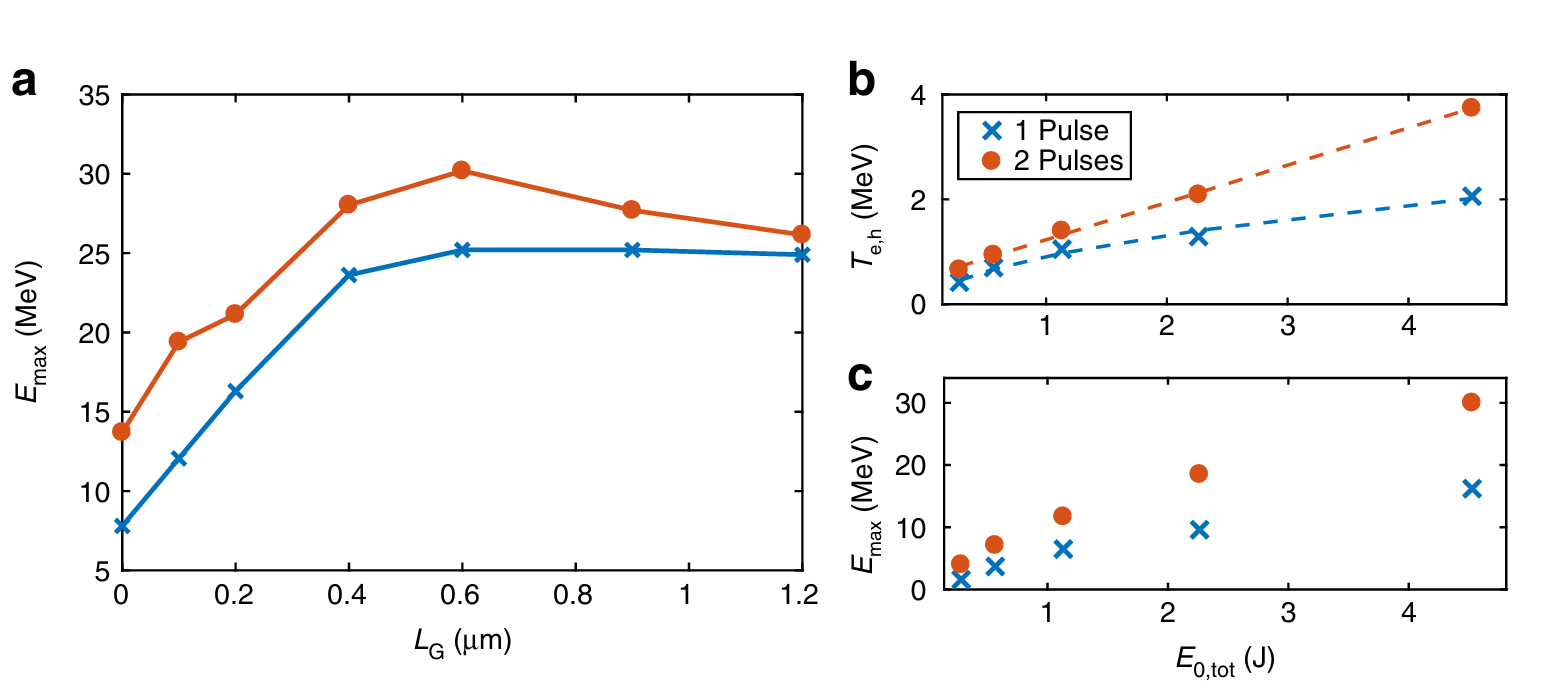
\includegraphics[width=\linewidth]{planning/images/ferri_scale_energy.PNG}
	\caption{Double pulse effectiveness in terms of changing preplasma scale length (a) and total laser energy (b,c) from Ferri et. al. (2019)\cite{Ferri_2019_Nat_Comm}.}
	\label{fig:ferri_scale_energy}
\end{figure}

Furthermore, Ferri performed some simulations that explored the effect of changing the preplasma scale length $L$ at a fixed energy, and changing the total laser energy for the flat target\cite{Ferri_2019_Nat_Comm} which can be seen in \cref{fig:ferri_scale_energy}. He finds that a higher preplasma scale length generally increases the max proton energy up to a certain scale length of around $L = \SI{0.6}{\micro \meter}$. Additionally, the enhancement is seen for all scale lengths, but the gap between single and pulse diminishes for larger scale lengths. In the double pulse case, a more favorable scaling with laser energy is seen for both the hot electron temperature and maximum proton energy ($E_\text{0,tot}$ as opposed to $\sqrt{E_\text{0,tot}}$) when comparing double pulse against single. In addition, Ferri comments that, for pulses with total energy greater than 10 J, the proton layer on the rear side starts to entirely disconnect from the bulk of the target during the acceleration, causing proton energies to saturate and become lower than the expected linear scaling.

\subsubsection{Other Simulations}
In 2021, eTNSA was again demonstrated through simulations in Rahman et. al.\cite{Rahman_2021_PoP} for a mJ class laser, around 2 orders of magnitude lower energy than the setup in Ferri's work. This mJ class laser is based on the experimental facility at the Wright Patterson Air Force Base (see \cref{ch:6} for more details) which utilizes a thinner target of $\sim \SI{460}{\nano \meter}$. Despite the major difference in laser and target parameters, the findings are similar -- increased hot electron temperature and proton energies with double pulse compared to single pulse. However, Rahman finds that the presence of a preplasma actually \emph{reduces} the maximum proton energy. But, like Ferri et. al., the gap between single and double pulse becomes smaller in the presence of a preplasma.

In 2024, Khan and Saxena\cite{Khan_2024_NJoP} revisit the double pulse scheme but with an applied longitudinal kilo-Tesla level magnetic field. The purpose of the magnetic field is to reduce the divergence of the hot electron beam. This guides the electrons and enhances the TNSA process to see a higher maximum cutoff energy in the proton spectrum\cite{Arefiev_2016_NJoP}. In this study, the laser was based off of the experimental set-up at the Rutherford Appleton Lab with a peak intensity of $\SI{5.5e20}{\watt \per \centi \meter \squared}$ incident on a $\SI{7}{\micro \meter}$ polyethelene target. 

% Preplasma is only on front of target just like titan dub pulse sims

\subsubsection{Experiments}

Due to multiple studies demonstrating eTNSA\cite{Ferri_2019_Nat_Comm,Rahman_2021_PoP,Khan_2024_NJoP}, experiments are needed to validate the PIC simulations. Morace et al.\cite{Morace_2019_Nat_Comm} showed that splitting a 270 J beam into multiple ``beamlets'' enhances the proton energy spectrum.

\begin{figure}
	\centering 
	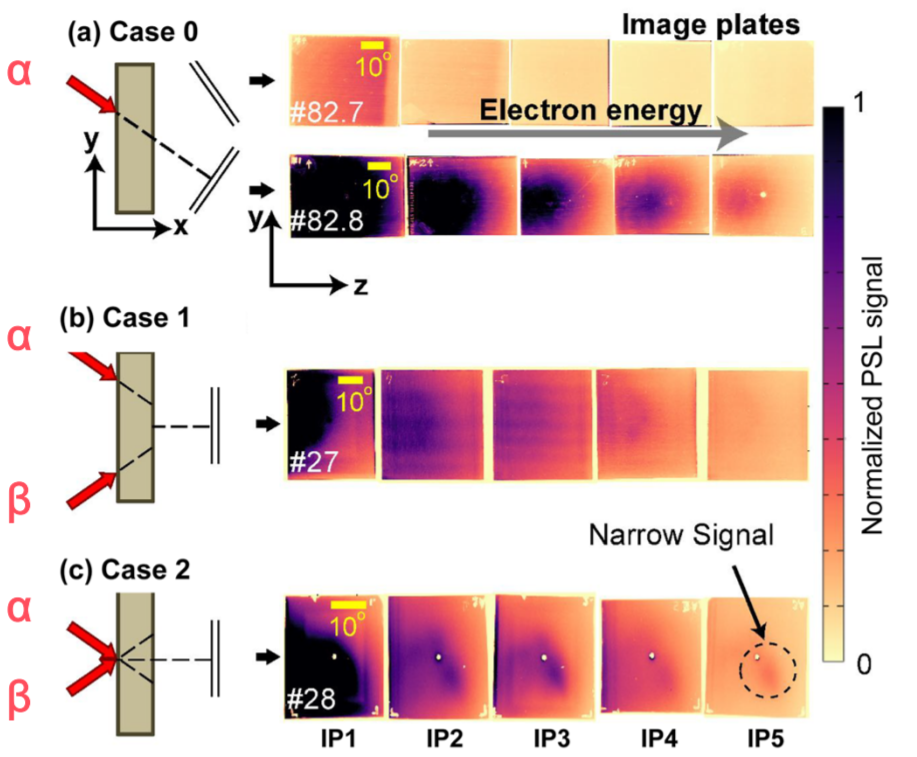
\includegraphics[width=\linewidth]{planning/images/yao_exp_stacks.PNG}
	\caption{FIG. 2 from Yao et al.\cite{Yao_2024_MaRaE}. Case 0 shows electron signals from a single pulse. Case 1 shows electron signals from a double pulse with spatial separation $\SI{120}{\micro \meter}$. Case 2 shows electron signals from a double pulse with no spatial separation.}
	\label{fig:yao_exp_stacks}
\end{figure}

Yao et al.\cite{Yao_2024_MaRaE} investigated the double pulse effect by changing the transverse spatial separation between two temporally aligned pulses as shown in \cref{fig:yao_exp_stacks}. This figure shows two possible beams $\alpha$ and $\beta$ which come in at equal and opposite incidence angles with $\alpha$ angled in the $-y$ direction. Comparing (b) and (c) shows an enhancement of the double pulse electron energy when the pulses are spatially overlapped. In (a), the electron energy is recorded along the laser beam axis in contrast to (b) and (c) and this shows that most the electrons are getting accelerated along the laser beam axis. 

%Explain RCF stacks
\section{Simulations}

\section{Discussion}

